\begin{XeClass}{FsStatus}
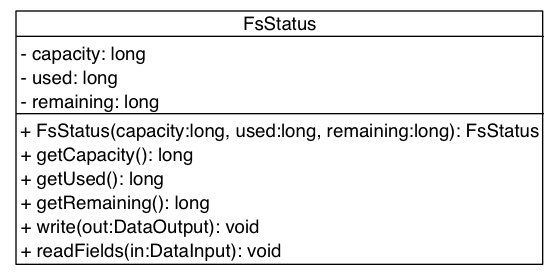
\includegraphics[width=10cm]{cdig/FsStatus.png}
     
 FsStatus是用于展示FileSystem的容量,空闲空间和使用空间的情况\emph{FileSystem}.
 FsStatus有三个私有成员变量,capacity,used,remaining
 并且引用Writable接口,实现write(DataOutput out)方法和readFields(DataInput in)方法

    \begin{XeMethod}{\XePublic}{FsStatus}{FsStatus}
         

    \end{XeMethod}

    \begin{XeMethod}{\XePublic}{long}{getCapacity}
         
 返回文件系统容纳字节数的容量

    \end{XeMethod}

    \begin{XeMethod}{\XePublic}{long}{getUsed}
         
 返回文件系统已经使用的字节数所占的空间大小

    \end{XeMethod}

    \begin{XeMethod}{\XePublic}{long}{getRemaining}
         
 返回文件系统剩下的字节数所占的空间大小

    \end{XeMethod}

    \begin{XeMethod}{\XePublic}{void}{write}
         
 分别将capacity,used,remaining的值写入输出流中,每个值由八个字节组成

    \end{XeMethod}

    \begin{XeMethod}{\XePublic}{void}{readFields}
         
 分别从输入流中读取capacity,used,remaining的值,每个值由八个字节组成

    \end{XeMethod}

\end{XeClass}
